\subsection{Vector-Valued Integrals and Curves}

\begin{definition} \label{def:vector-valued-riemann-stieltjes-integral} \hlt{Vector-Valued Riemann--Stieltjes Integral}\\
Let $a,b\in\R$ satisfy $a<b$, $k\in\N$, $\alpha:[a,b]\to\R$ increasing. For $\mathbf{f}=(f_1,\ldots,f_k):[a,b]\to\R^k$, $\mathbf{f}\in\mathcal{R}(\alpha)$ iff $(\forall j\in\{1,\ldots,k\})\,f_j\in\mathcal{R}(\alpha)$.\\
In that case, set $\int_a^b\mathbf{f}\,d\alpha\defeq\left(\int_a^b f_1\,d\alpha,\ldots,\int_a^b f_k\,d\alpha\right)$. For the identity integrator $t\mapsto t$, write $\mathbf{f}\in\mathcal{R}[a,b]$ and $\int_a^b\mathbf{f}(t)\,dt$.
\end{definition}

\begin{theorem} \label{thm:vector-valued-integral-results} \hlt{Vector-Valued Integral Results}\\
Let $a,b\in\R$ satisfy $a<b$, $k\in\N$. For Parts (ii)--(iii), let $\alpha:[a,b]\to\R$ be increasing and let $\mathbf{f}\in\mathcal{R}(\alpha)$. Then:
\begin{enumerate}[label=(\roman*)]
\setlength{\itemsep}{0pt}
\item Let $\mathbf{g},\mathbf{F}:[a,b]\to\R^k$, where $\mathbf{g}\in\mathcal{R}[a,b]$ and $\mathbf{F}$ is continuous on $[a,b]$ and differentiable on $(a,b)$.\\
If $(\forall t\in(a,b))\,\mathbf{F}'(t)=\mathbf{g}(t)$, then $\int_a^b\mathbf{g}(t)\,dt=\mathbf{F}(b)-\mathbf{F}(a)$.
\item The map $t\mapsto\norm{\mathbf{f}(t)}$ belongs to $\mathcal{R}(\alpha)$.
\item $\norm{\int_a^b\mathbf{f}\,d\alpha}\leq\int_a^b\norm{\mathbf{f}(t)}\,d\alpha$.
\end{enumerate}
\begin{proof}
\begin{enumerate}[label=(\roman*)]
\setlength{\itemsep}{0pt}
\item Write $\mathbf{g}=(g_1,\ldots,g_k)$ and $\mathbf{F}=(F_1,\ldots,F_k)$. By Definition \ref{def:vector-valued-riemann-stieltjes-integral}, $(\forall j\in\{1,\ldots,k\})\,g_j\in\mathcal{R}[a,b]$.\\
Maps $F_1,\ldots,F_k$ continuous on $[a,b]$ by Theorem \ref{thm:continuous-algebra-and-components}(ii). $(\forall j\in\{1,\ldots,k\})(\forall t\in(a,b))\,F_j'(t)=g_j(t)$ by Proposition \ref{prop:vector-derivative-componentwise}.\\
Thus $(\forall j\in\{1,\ldots,k\})\,\int_a^b g_j(t)\,dt=F_j(b)-F_j(a)$ by Theorem \ref{thm:fundamental-theorem-calculus-riemann}. The vector identity follows by Definition \ref{def:vector-valued-riemann-stieltjes-integral}.
\item Write $\mathbf{f}=(f_1,\ldots,f_k)$, $q\defeq\sum\limits_{j=1}^{k}f_j^2$. Then $q\in\mathcal{R}(\alpha)$ by Theorem \ref{thm:products-and-absolute-values-riemann-stieltjes}(i) and Theorem \ref{thm:riemann-stieltjes-integral-properties}(i).\\
Choose $M\geq0$ with $q([a,b])\subseteq[0,M]$ by Definition \ref{def:riemann-stieltjes-integral}. Since $(\forall t\in[a,b])\,\norm{\mathbf{f}(t)}=\sqrt{q(t)}$, claim follows by Theorem \ref{thm:continuous-composition-preserves-riemann-stieltjes-integrability}.
\item Set $\mathbf{y}\defeq\int_a^b\mathbf{f}\,d\alpha$. If $\mathbf{y}=\mathbf{0}$,  claim holds by Part (ii) and Theorem \ref{thm:riemann-stieltjes-integral-properties}(ii) with zero function.\\
Suppose $\mathbf{y}\neq\mathbf{0}$, $\mathbf{u}\defeq\mathbf{y}/\norm{\mathbf{y}}$, $h(t)\defeq\mathbf{u}\cdot\mathbf{f}(t)$. Then $h\in\mathcal{R}(\alpha)$ by Definition \ref{def:vector-valued-riemann-stieltjes-integral} and Theorem \ref{thm:riemann-stieltjes-integral-properties}(i).\\
Since $\norm{\mathbf{u}}=1$, $(\forall t\in[a,b])\,h(t)\leq\abs{h(t)}\leq\norm{\mathbf{f}(t)}$ by Theorem \ref{thm:cauchy-schwarz-inequality}(i).\\
Moreover, $\int_a^b h\,d\alpha=\mathbf{u}\cdot\mathbf{y}=\norm{\mathbf{y}}$ by Definition \ref{def:vector-valued-riemann-stieltjes-integral}, Theorem \ref{thm:riemann-stieltjes-integral-properties}(i). Claim follows by Theorem \ref{thm:riemann-stieltjes-integral-properties}(ii).
\end{enumerate}
\hlt{Structural Commentary}: Coordinates prove the antiderivative formula; norm composition and unit projection prove the norm claims.\\
\hlt{Key Insight}: Normalize the integral vector before applying scalar order.
\end{proof}
\end{theorem}

\begin{definition} \label{def:curves-and-rectifiability} \hlt{Curves and Rectifiability}\\
Let $a,b\in\R$ satisfy $a<b$, and let $k\in\N$.
\begin{enumerate}[label=(\roman*)]
\setlength{\itemsep}{0pt}
\item A \hlt{curve} in $\R^k$ is a continuous map $\gamma:[a,b]\to\R^k$.\\
The curve $\gamma$ is an \hlt{arc} iff $\gamma$ is injective; it is a \hlt{closed curve} iff $\gamma(a)=\gamma(b)$.
\item For a partition $\Pi=\{a=x_0<\cdots<x_n=b\}$, set $\ell(\Pi,\gamma)\defeq\sum\limits_{i=1}^{n}\norm{\gamma(x_i)-\gamma(x_{i-1})}$.
\item The \hlt{length} of $\gamma$ is $\ell(\gamma)\defeq\sup\limits_{\Pi}\ell(\Pi,\gamma)\in[0,+\infty]$, where $\Pi$ ranges over all partitions of $[a,b]$. The curve $\gamma$ is \hlt{rectifiable} iff $\ell(\gamma)<+\infty$.
\end{enumerate}
\end{definition}

\begin{perspective} \label{per:length-is-not-position-limit} \hlt{Length Is Not Just Shape}\\
For $N\in\N\setminus\{0\}$, set $v_{2i}\defeq(\frac{i}{N},\frac{i}{N})$ for $0\leq i\leq N$ and $v_{2i+1}\defeq(\frac{i+1}{N},\frac{i}{N})$ for $0\leq i<N$.\\
Let $\gamma_N:[0,1]\to\R^2$ satisfy $\gamma_N(\frac{m}{2N})=v_m$ for $0\leq m\leq2N$ and be affine on each intervening subinterval.\\
Its $2N$ segments have length $\frac{1}{N}$, so $\ell(\gamma_N)=2$, while its range lies within distance $\frac{1}{N}$ of the diagonal chord.\\
The chord has length $\sqrt{2}$; closeness of curve ranges therefore does not control length.
\end{perspective}

\noindent Figure \ref{fig:staircase-length-vs-chord} depicts the case $N=6$ from Perspective \ref{per:length-is-not-position-limit}.
\begin{illustrationfigure}[H]
  \centering
  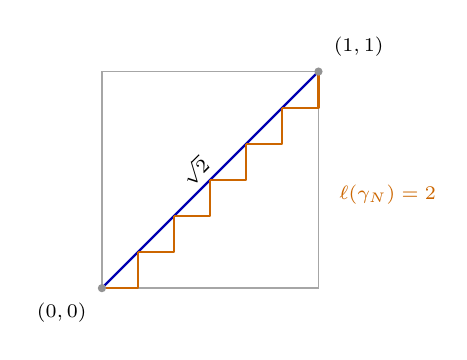
\begin{tikzpicture}[
  scale=2.75,
  every node/.style={font=\scriptsize},
  side/.style={gray!70, line width=0.55pt},
  chord/.style={blue!70!black, line width=0.85pt},
  stair/.style={orange!80!black, line width=0.8pt, line join=round},
  point/.style={circle, fill=gray!85, inner sep=1.05pt},
  labelbox/.style={fill=white, fill opacity=0.88, text opacity=1, inner sep=1.1pt}
]
  \coordinate (A) at (0,0);
  \coordinate (B) at (1,1);

  \draw[side] (0,0) rectangle (1,1);

  \draw[chord] (A) -- (B);

  \foreach \i in {0,...,5} {
    \draw[stair] ({\i/6},{\i/6}) -- ({(\i+1)/6},{\i/6}) -- ({(\i+1)/6},{(\i+1)/6});
  }

  \node[point] at (A) {};
  \node[point] at (B) {};
  \node[below left=2pt] at (A) {$(0,0)$};
  \node[above right=2pt] at (B) {$(1,1)$};

  \node[labelbox, rotate=45] at (0.43,0.54) {$\sqrt{2}$};
  \node[orange!80!black, labelbox, anchor=west] at (1.08,0.43) {$\ell(\gamma_N)=2$};
\end{tikzpicture}

  \caption{The six-step staircase has length $2$, while the diagonal chord has length $\sqrt{2}$.}
  \label{fig:staircase-length-vs-chord}
\end{illustrationfigure}

\begin{theorem} \label{thm:continuously-differentiable-curves-rectifiable} \hlt{Length of a Continuously Differentiable Curve}\\
Let $a,b\in\R$ satisfy $a<b$, let $k\in\N$, and let $\gamma:[a,b]\to\R^k$ be a curve differentiable relative to $[a,b]$.\\
If $\gamma':[a,b]\to\R^k$ is continuous, then $\gamma$ is rectifiable, with $\ell(\gamma)=\int_a^b\norm{\gamma'(t)}\,dt$.
\begin{proof}
\begin{enumerate}[label=(\roman*)]
\setlength{\itemsep}{0pt}
\item \hlt{Integrability}: Write $\gamma'=(g_1,\ldots,g_k)$. Then $(\forall j\in\{1,\ldots,k\})\,g_j$ is continuous by Theorem \ref{thm:continuous-algebra-and-components}(ii).\\
Thus $(\forall j\in\{1,\ldots,k\})\,g_j\in\mathcal{R}[a,b]$ by Theorem \ref{thm:continuous-functions-riemann-stieltjes-integrable} with the identity integrator, so $\gamma'\in\mathcal{R}[a,b]$ by Definition \ref{def:vector-valued-riemann-stieltjes-integral}.\\
Set $\rho\defeq(t\mapsto\norm{\gamma'(t)})$. Then $\rho\in\mathcal{R}[a,b]$ by Theorem \ref{thm:vector-valued-integral-results}(ii); set $L\defeq\int_a^b\rho(t)\,dt$.
\item \hlt{Upper Bound}: Fix a partition $\Pi=\{a=x_0<\cdots<x_n=b\}$ and set $\Delta\gamma_i\defeq\gamma(x_i)-\gamma(x_{i-1})$.\\
Then $(\forall i\in\{1,\ldots,n\})\,\norm{\Delta\gamma_i}\leq\int_{x_{i-1}}^{x_i}\rho(t)\,dt$ by Theorem \ref{thm:vector-valued-integral-results}(i),(iii).\\
Thus $\ell(\Pi,\gamma)\leq L$ by Theorem \ref{thm:riemann-stieltjes-integral-properties}(iii) with the identity integrator. Hence $\ell(\gamma)\leq L<+\infty$ by Definition \ref{def:curves-and-rectifiability}, so $\gamma$ is rectifiable.
\item \hlt{Local Reverse Bound}: Fix $\varepsilon>0$. Choose $\delta>0$ such that $(\forall s,t\in[a,b])\,[\abs{s-t}<\delta\Rightarrow\norm{\gamma'(s)-\gamma'(t)}<\varepsilon]$ by Theorem \ref{thm:compact-continuity-uniform-continuity}.\\
Choose a partition $\Pi=\{a=x_0<\cdots<x_n=b\}$ with $\operatorname{mesh}(\Pi)<\delta$. Set $\mathbf{v}_i\defeq\gamma'(x_{i-1})$ and $\Delta\gamma_i\defeq\gamma(x_i)-\gamma(x_{i-1})$ for $1\leq i\leq n$.\\
Then $(\forall i\in\{1,\ldots,n\})(\forall t\in[x_{i-1},x_i])\,\norm{\gamma'(t)-\mathbf{v}_i}<\varepsilon$ by the choice of $\delta$.\\
The identities $(\forall i\in\{1,\ldots,n\})\,\mathbf{v}_i\Delta x_i-\Delta\gamma_i=\int_{x_{i-1}}^{x_i}[\mathbf{v}_i-\gamma'(t)]\,dt$ hold by Theorem \ref{thm:vector-valued-integral-results}(i).\\
Hence $(\forall i\in\{1,\ldots,n\})\,\norm{\mathbf{v}_i\Delta x_i-\Delta\gamma_i}\leq\varepsilon\Delta x_i$ by Theorem \ref{thm:vector-valued-integral-results}(iii), Theorem \ref{thm:riemann-stieltjes-integral-properties}(ii), and the pointwise bound.\\
The bounds $(\forall i\in\{1,\ldots,n\})(\forall t\in[x_{i-1},x_i])\,\rho(t)\leq\norm{\mathbf{v}_i}+\varepsilon$ hold by Theorem \ref{thm:triangle-inequality-inner-product}(i).\\
Thus $(\forall i\in\{1,\ldots,n\})\,\int_{x_{i-1}}^{x_i}\rho(t)\,dt\leq\norm{\Delta\gamma_i}+2\varepsilon\Delta x_i$ by Theorem \ref{thm:riemann-stieltjes-integral-properties}(ii), Theorem \ref{thm:triangle-inequality-inner-product}(i), and the preceding bound.
\item \hlt{Conclusion}: $L\leq\ell(\Pi,\gamma)+2\varepsilon(b-a)\leq\ell(\gamma)+2\varepsilon(b-a)$ by Theorem \ref{thm:riemann-stieltjes-integral-properties}(iii) with the identity integrator and Definition \ref{def:curves-and-rectifiability}.\\
Since $\varepsilon>0$ is arbitrary, $L\leq\ell(\gamma)\leq L$, so $\ell(\gamma)=L$.
\end{enumerate}
\hlt{Structural Commentary}: Vector integration bounds polygonal sums; uniform derivative control reverses the estimate on fine partitions.\\
\hlt{Key Insight}: Short chords approximate their constant-velocity integrals.
\end{proof}
\end{theorem}
